\chapter{Social network visualization}

Even though the data mining processes described in the previous chapters give us valuable insights into the structure of social networks, 
they are not necessarily easy to interpret for laymen.
One way to make the results of data mining more accessible is to create data visualization, that is present the data with their visual representation, 
while using different visual cues to guide the viewers' attention towards different qualities.

In this part of the thesis, we will assess the current state of the visualizations in the Charles Explorer application, 
will propose some improvements to make the visualization more accessible to the users and will implement those.

At the moment of publishing this thesis, the person search mode in the Charles Explorer application\footnote{Available e.g. at \url{https://explorer.cuni.cz/person/1732969562160398}} already contains the experimental prototype of the changes proposed in this chapter.
For consistency, we will still consider the ``current state'' of the visualization the one \textit{without} the proposed changes.

The implementation of the visualization components is available in the GitLab repository\footnote{At \url{https://gitlab.mff.cuni.cz/barj/charles-explorer/}}.

\section{Vocabulary}

This section introduces some basic vocabulary that we will use throughout this chapter.

\textbf{Ego network}: Ego-centric networks (or shortened to “ego” networks) are particular networks which specifically map the connections of and from the perspective of a single person (an “ego”). (\cite{Lizardo2020-xo})

\textbf{Visual decoding}: Also called \textit{preattentive processing} or \textit{preattentive vision}, visual decoding is the instantaneous perception of the visual field that comes without apparent mental effort. (\cite{Cleveland1985})

\textbf{Node contraction}: Since we will be working with bipartite graphs, we will use the term \textit{node contraction} to denote the process of replacing a node from one partition with edges between all the incident nodes from the other partition.
This is effectively \textit{path contraction} for paths of length $2$.

\section{Assessing the current state} \label{sec:current-state}

The current state of the Charles Explorer visualization views is quite simple. 

In the \textit{Person} search mode, the user can search for people inside the Charles University. 
When accessing a person's profile, the application shows the person's \textit{ego network} with the main person and their direct collaborators 
as nodes and their common publications aggregated to the edges.

\begin{figure}[ht!]
    \captionsetup{width=.9\linewidth}
    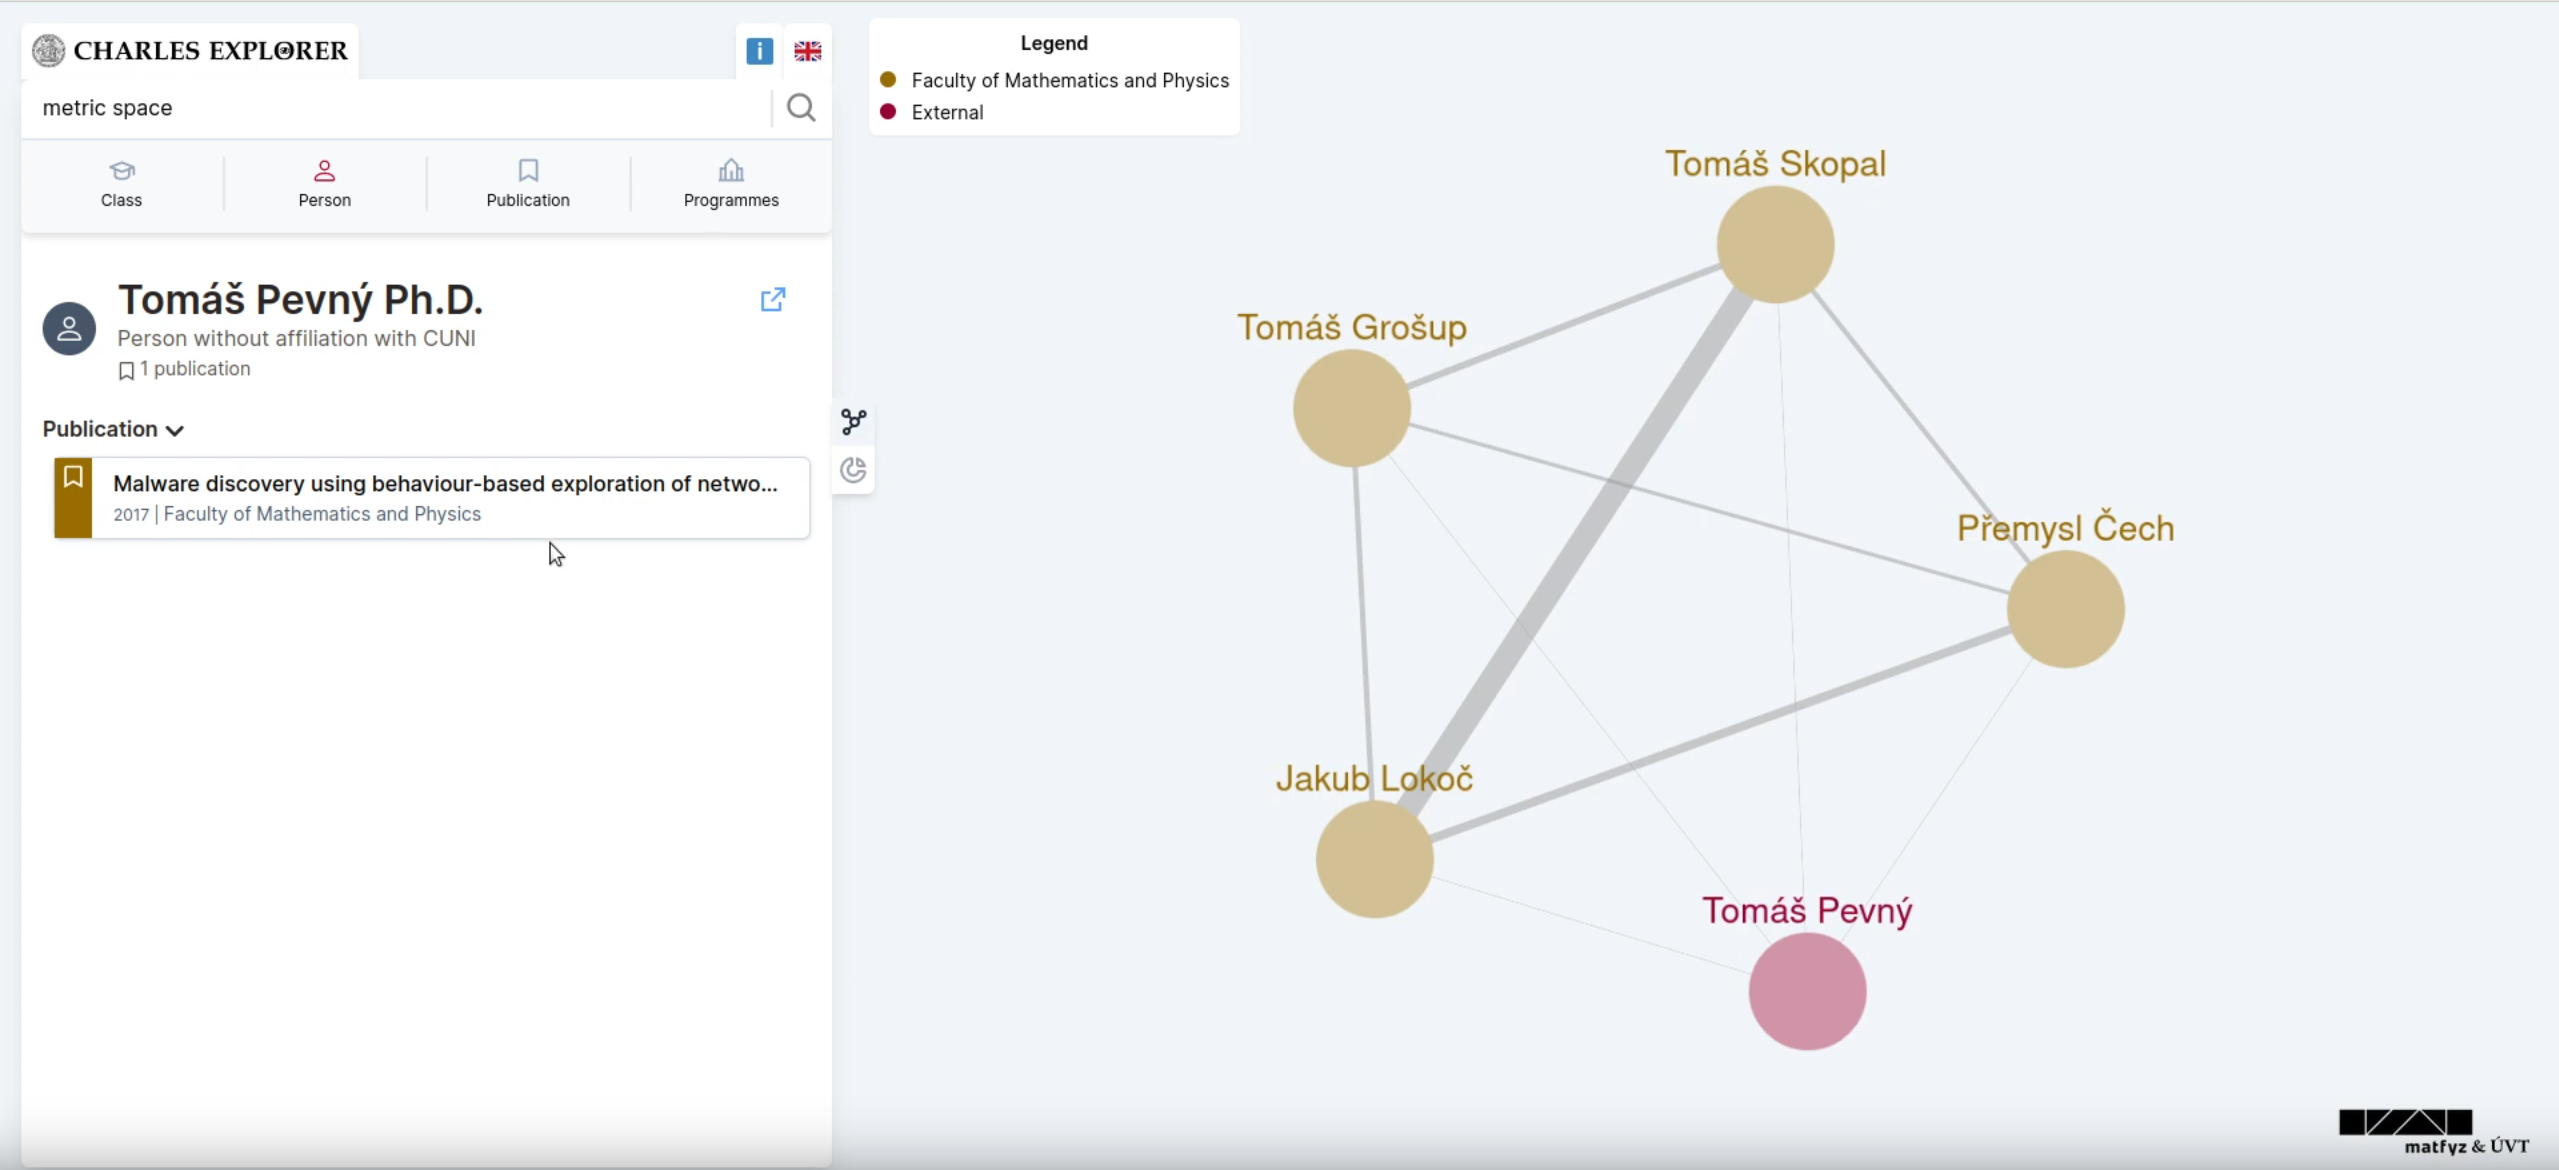
\includegraphics[width=0.8\textwidth]{../img/charles-explorer-old-view.png}
    \centering
    \caption{Charles Explorer showing the \textit{ego network} of a person.}
\end{figure}

The graph is displayed with force-directed layout. The edge thickness is proportional to the number of common publications between 
the two people and the colors of the nodes represent the person's faculty association.

This approach has multiple drawbacks which we will now discuss.

\subsection{Problems with color coding} \label{sec:color-coding}

Firstly, the color coding of the nodes does not prove useful, as it hinders the \textit{visual decoding} of the graph.
The user spends attention on reading the legend, rather than interpreting the graph subconciously.

This is especially true for larger ego networks with many nodes with different faculty affiliations. 
Additionaly, the application does not provide any alternative visual cue for color vision deficient users.

\begin{figure}[ht!]
    \captionsetup{width=.9\linewidth}
    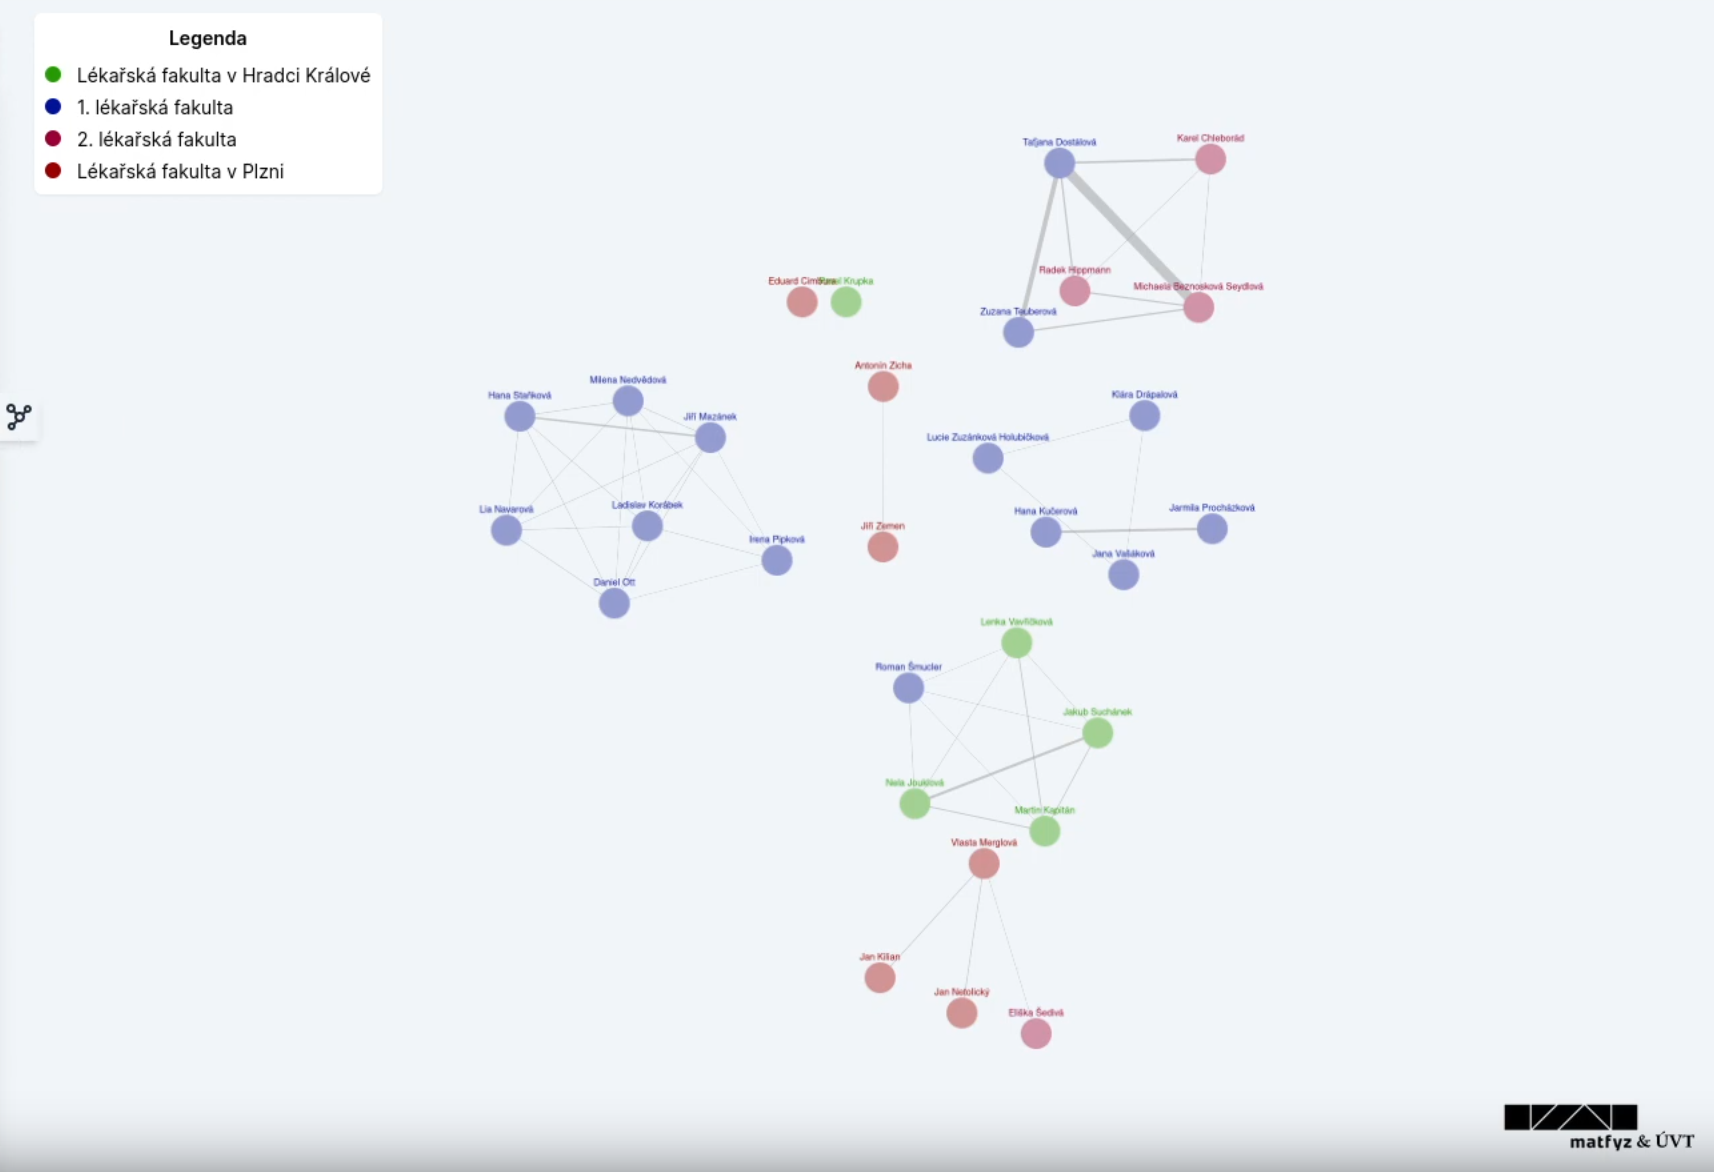
\includegraphics[width=0.7\textwidth]{../img/color-coding.png}
    \centering
    \caption{Graph view for query \textit{`dentistry'} shows nodes with various faculty affiliations.}
\end{figure}

According to \cite{Cleveland1985}, the upper bound on color discrimination in one figure is 5–6 colors for a healthy viewer. 
This is not enough for the 17 faculties and departments of the Charles University. 
With faculties, there is also little room for a meaningful aggregation (of more faculties into one color), as the faculty structure is not hierarchical.

\subsection{Layouting problems} \label{sec:layouting-problems}

The arbitrary positions of the nodes based on the physical simulation layout increase the cognitive load 
of the viewer and contribute to the graph's worse readability.

\cite{munzner2015visualization} states that the position of data points on a common scale is the most effective way to communicate the data to the viewer.
By using the physical simulation layout, we are willingly giving up this visual channel (the \texttt{x} and \texttt{y} position of the nodes in the screen space).

In case the user is looking for a specific person in the graph, they have to scan the whole graph to find the person, as the node position does not code any inherent information about the person.

\subsection{Contracting publication nodes into edges}

The current data visualization uses authors as the nodes and contracts publications as the edges.
The number of common publications is aggregated to the edge thickness. \cite{10.5555/2385879} considers thickness a visual channel with a limited quantitative resolution.

Setting the edge width in proportion to the number of common publications might also cause confusion, as the \textit{area} of the edge depends both on the width and the length of the edge.
Longer edges might appear more important than the shorter ones, even though they might denote the same number of common publications.

This is undesirable, as it goes against the underlying idea of the physical simulation layout, which places the nodes closer to each other if they are more connected.

Furthermore, the contraction of the publication nodes into edges poses another problem.
A publication with $n$ authors contributes to $\frac{n(n-1)}{2}$ edges between its authors. 

\begin{figure}[ht!]
    \captionsetup{width=.9\linewidth}
    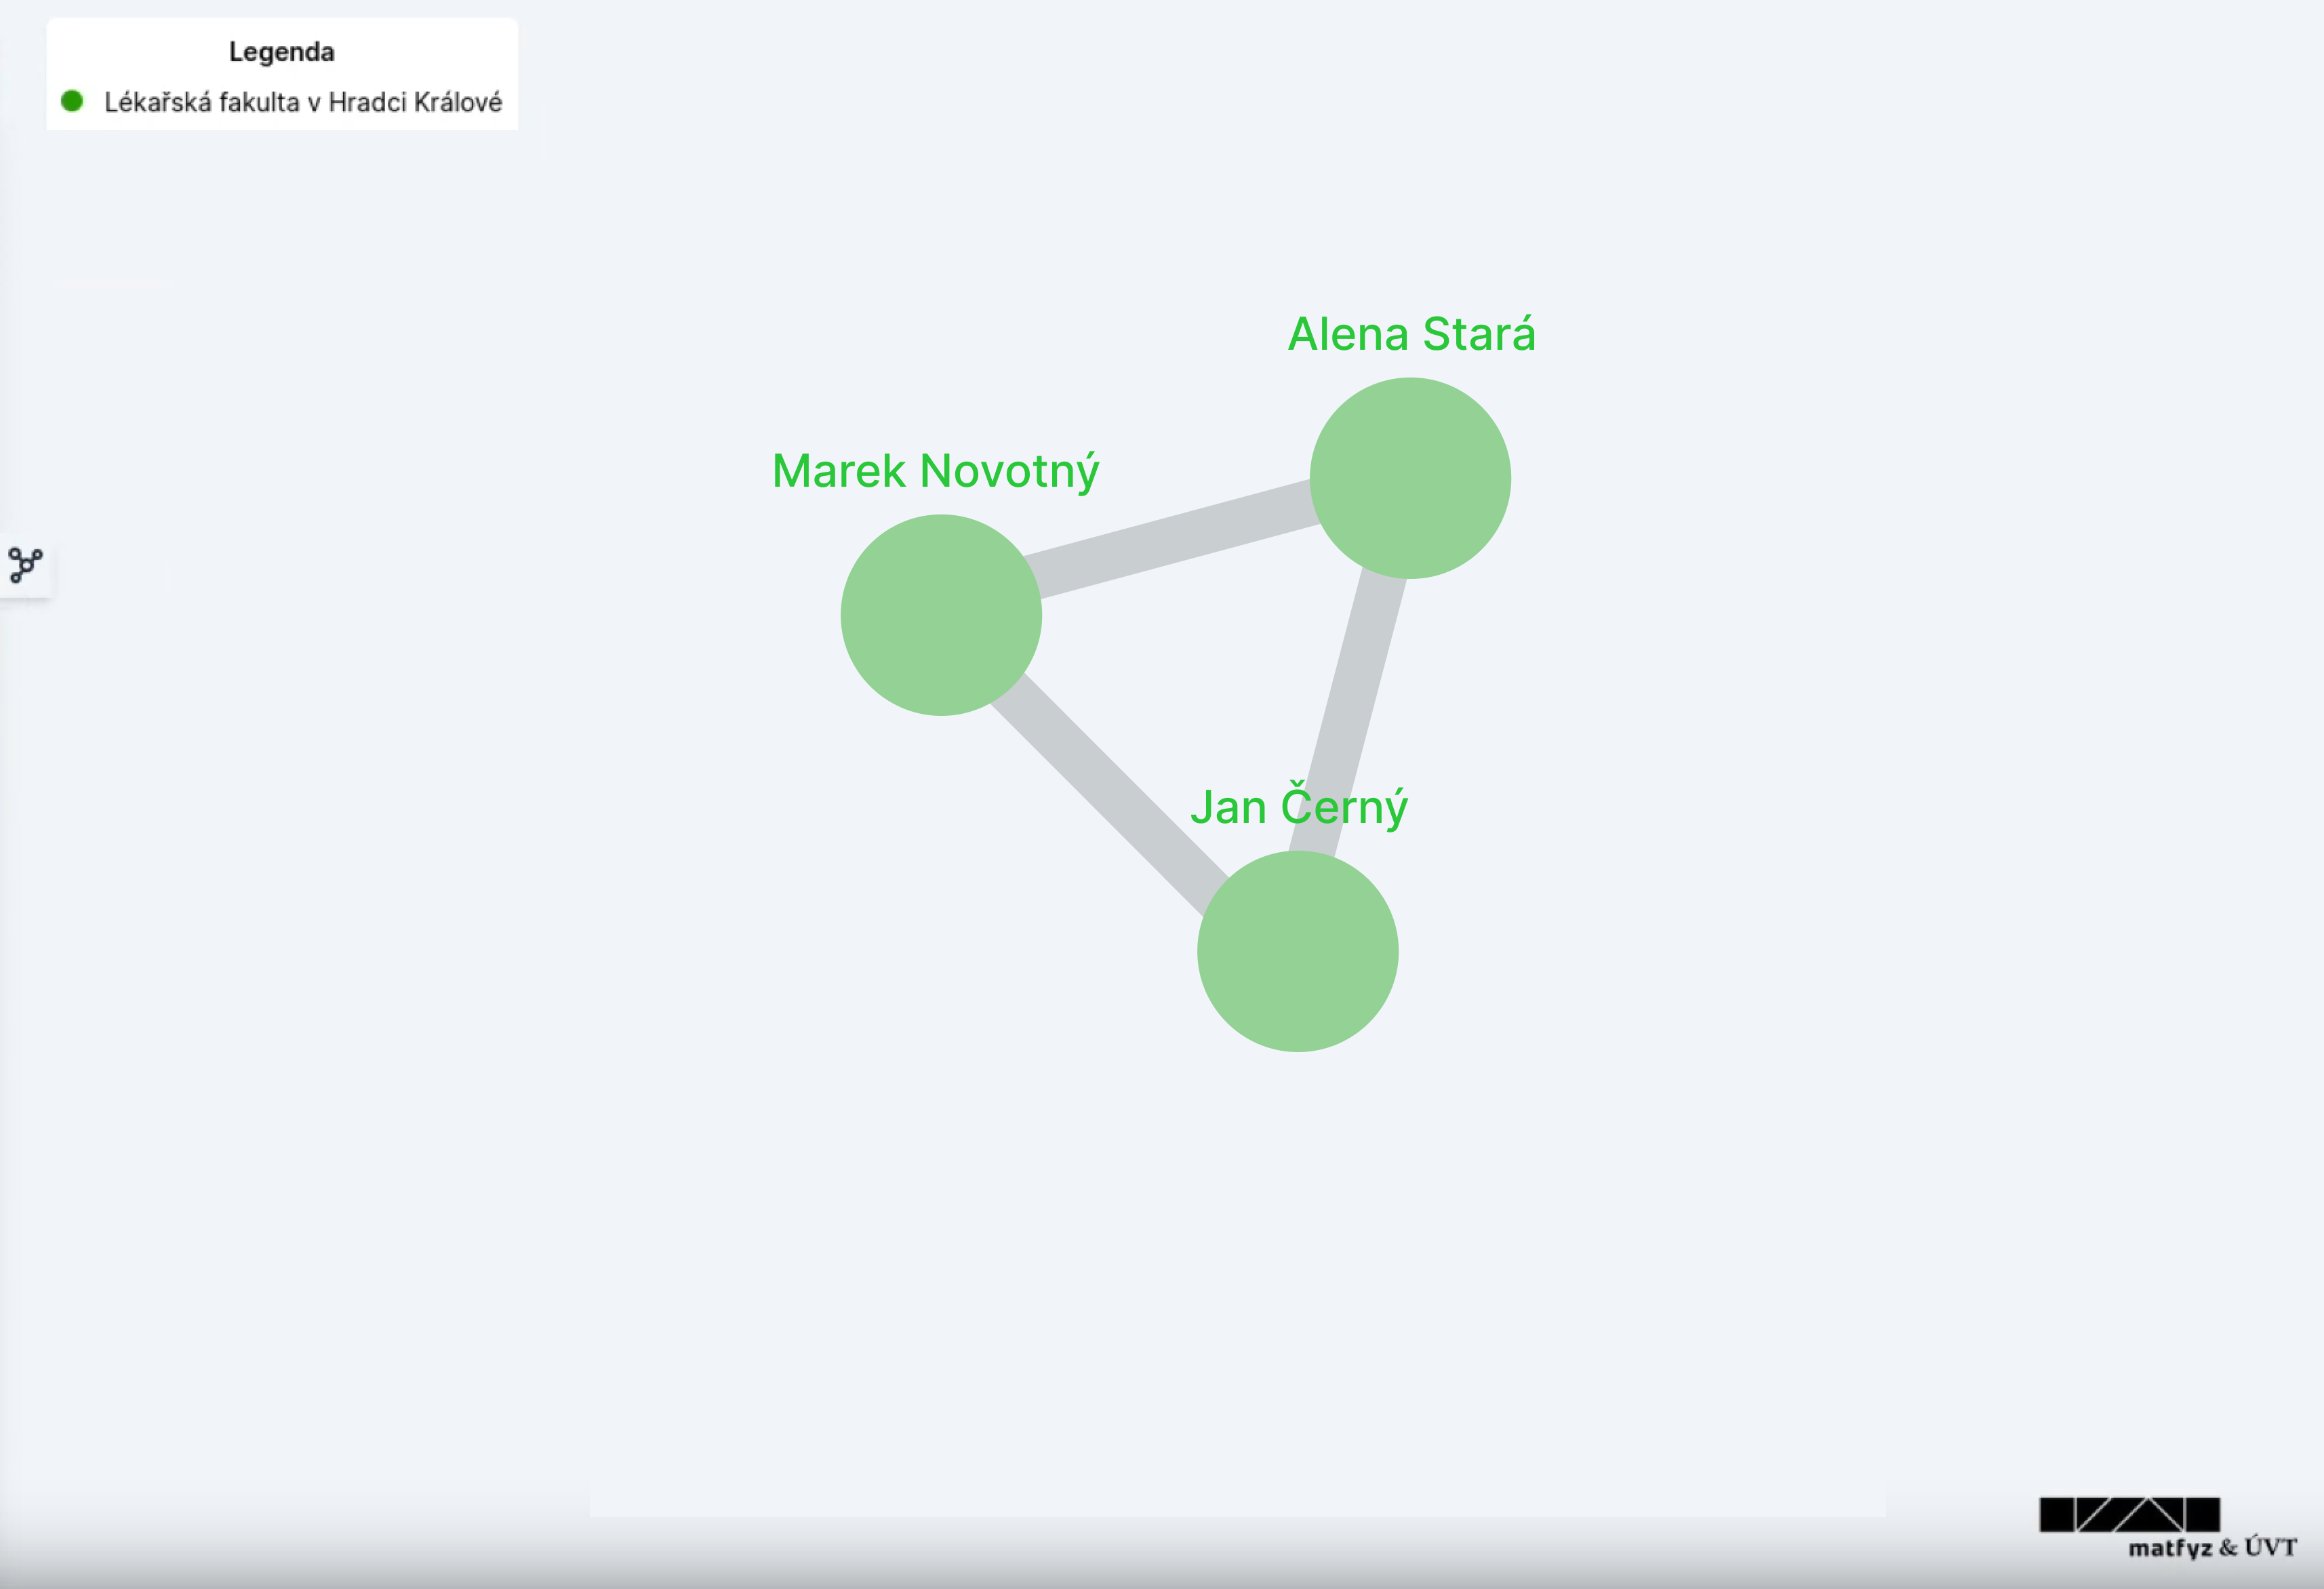
\includegraphics[width=0.7\textwidth]{../img/contraction.png}
    \centering
    \caption{Contracting publication nodes into edges only shows coauthorship between pairs of authors. Larger communities of coauthors (\# coauthors > 2) are not displayed correctly in the graph.}
\end{figure}

This means that publications with one author are not represented in the graph at all, as there are no edges to draw between the nodes.

For publications with more than two authors, one publication is represented by multiple edges between all the pairs of the authors.
This clutters the graph with edges and makes the publication - edge mapping less readable. 
For correct representation of those publications, we would need to draw hyperedges between the nodes, which might cause the readability of the graph to decrease even further.

\section{Addressing the issues}

To address the problems from the section \ref{sec:current-state} and improve the visualization of the ego networks, we propose changes to the current visualization.
We also implement an experimental prototype visualization of the proposed changes.

\subsection{Ego-network visualization}

To start, we can address the problem of the \textit{publication-edge contraction} by displaying the publications as nodes in the graph.

This way, both the entity types (authors and publications) are displayed as \textit{nodes} in the visualization.
This is perhaps easier to understand for a layman, as both authors and publications are real-life entities. 
The edges between the nodes now represent an incidence relation between the two entities.

The resulting graph is a bipartite graph, with two types of nodes - authors and publications, and edges connecting the authors to the publications they have co-authored.

To support the \textit{visual decoding} of the graph, we distinguish the two types of nodes by their shape. 
This way, the user can easily distinguish between the authors and the publications, even if they are color vision deficient 
or are viewing the visualization reproduced using a monochrome display medium (for example a print from a black-and-white printer).

The main node (the ego) is highlighted with color fill - since it is the only node of this type in the graph,
it is easy to distinguish from the other nodes - even with monochrome display mediums or color vision impairments.

\begin{figure}[ht!]
    \captionsetup{width=.9\linewidth}
    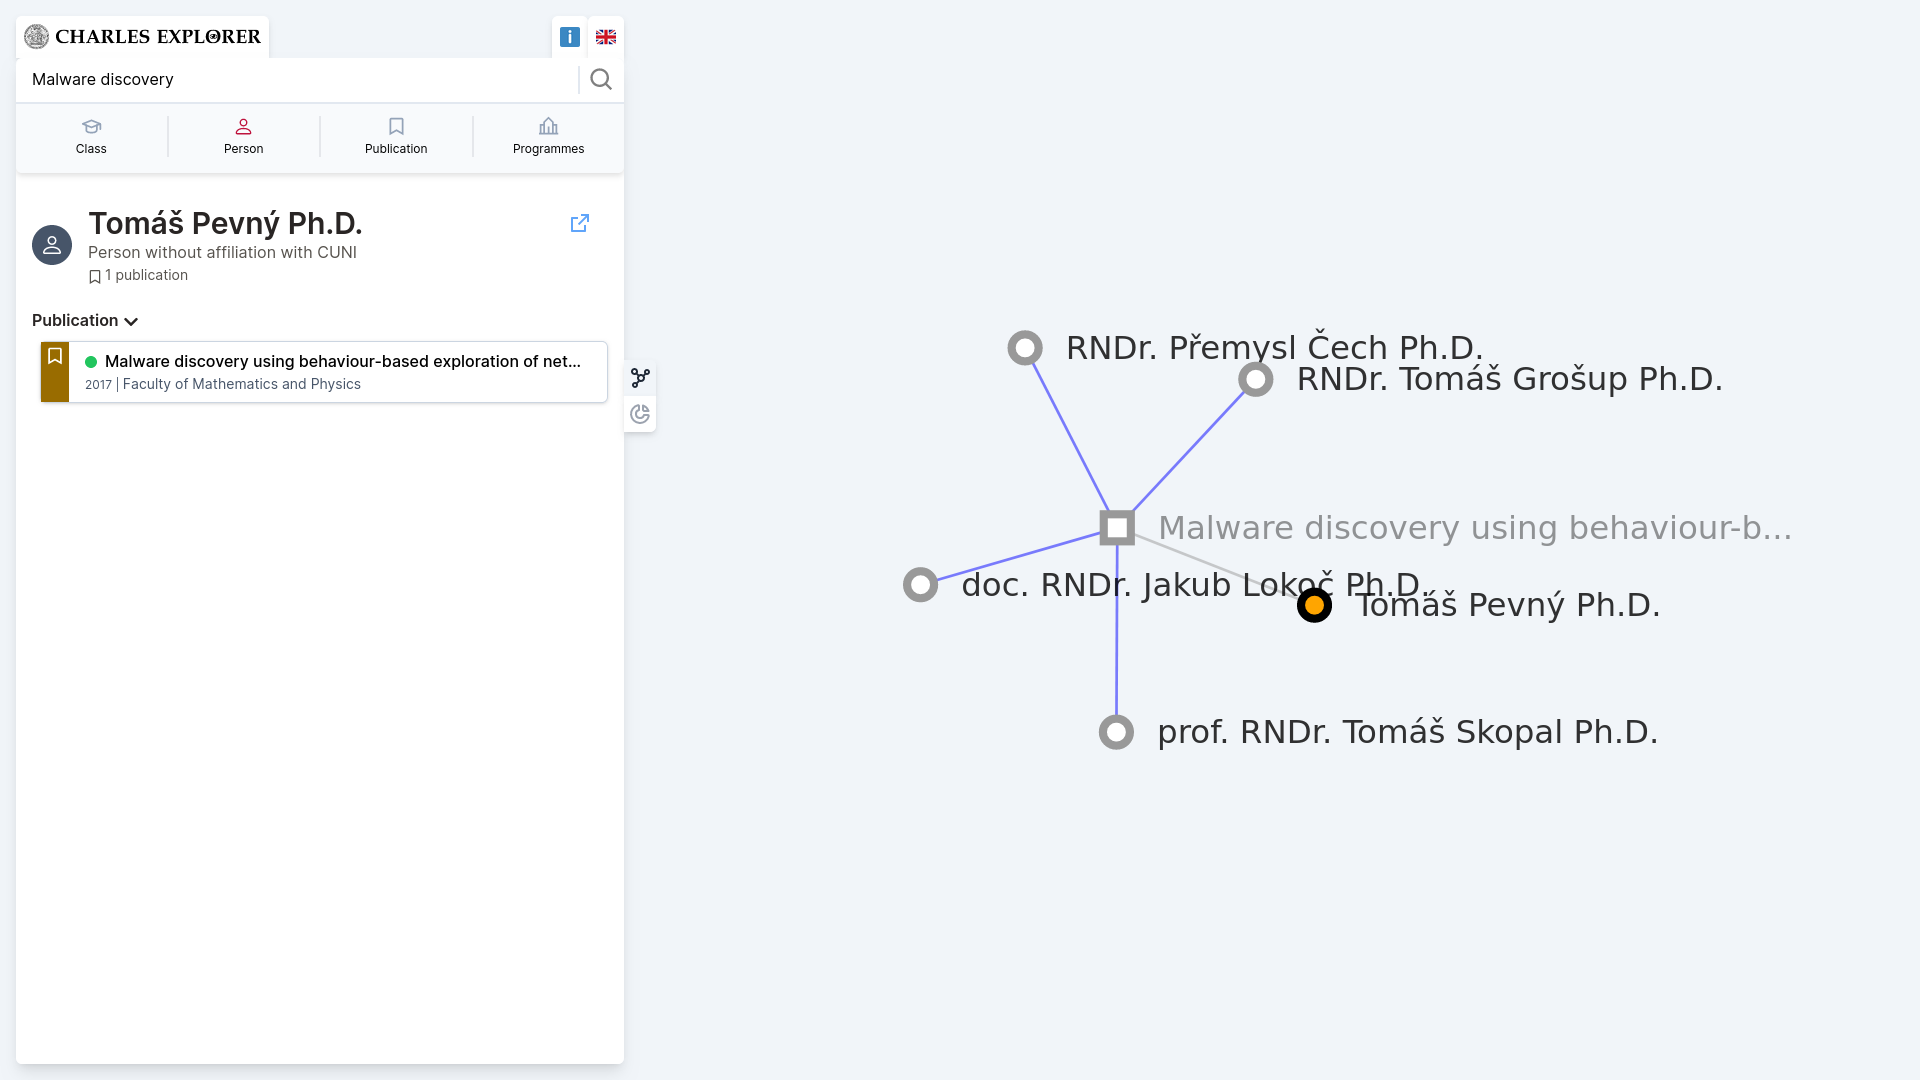
\includegraphics[width=0.7\textwidth]{../img/publications-and-people.png}
    \centering
    \caption{In the proposed visualization, the publications are displayed as nodes in the graph. \textit{Larger-than-binary} coauthorships are now represented correctly.}
\end{figure}

This approach also removes the need for the edge-width encoding of the number of common publications.

To avoid the color coding problems from \ref{sec:color-coding}, we defer the faculty affiliation information to the node tooltip.
This is only visible after the user hovers over the node with the mouse cursor, so it does not clutter the graph view.

\subsection{Node locality and layouting}

As mentioned in \ref{sec:layouting-problems}, the arbitrary positions of the nodes in the force-directed layout increase the cognitive load of the viewer.
For larger graphs, the viewer might not be able to find the node they are looking for, as the node position does not code any inherent information about the person.

To address this, we propose a search tool which highlights the search results in the graph.

\begin{figure}[ht!]
    \captionsetup{width=.9\linewidth}
    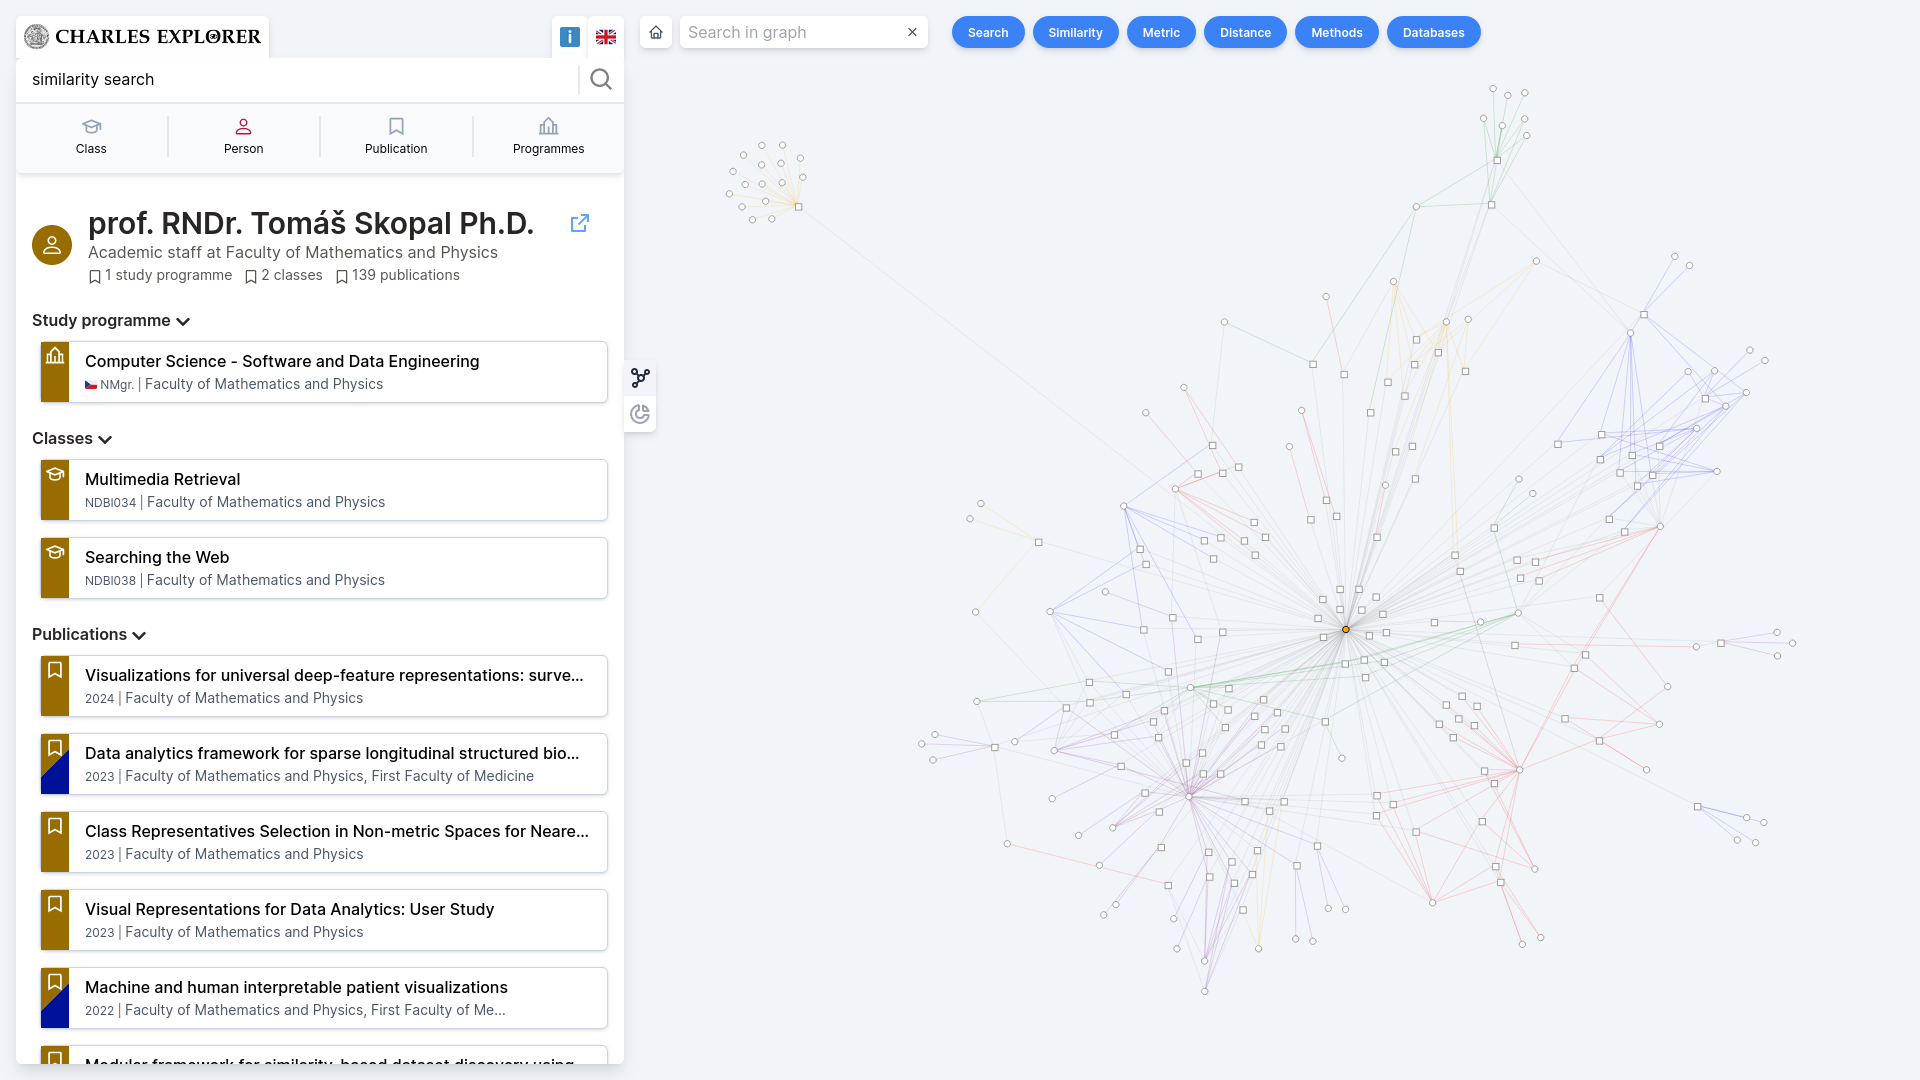
\includegraphics[width=0.8\textwidth]{../img/big-network.png}
    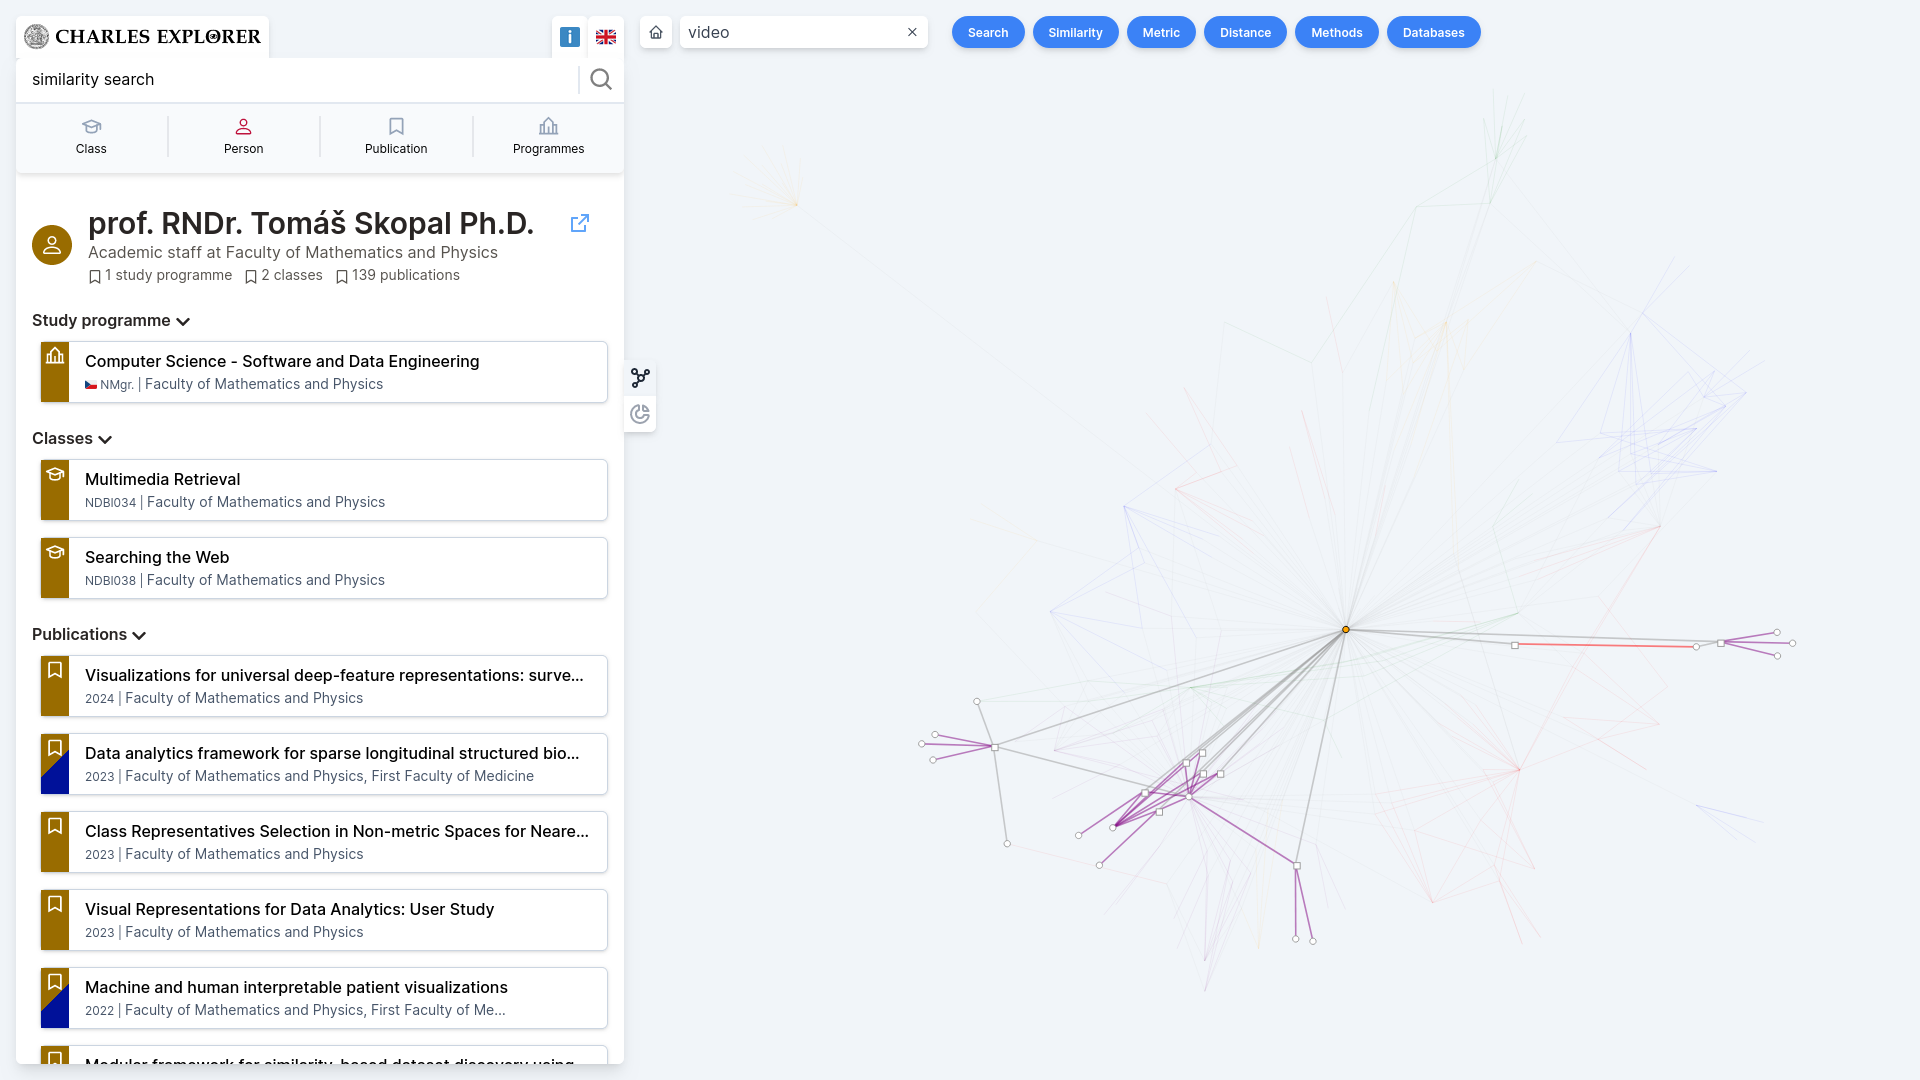
\includegraphics[width=0.8\textwidth]{../img/big-network-search.png}
    \centering
    \caption{The first picture shows a large ego network with many nodes. The second picture shows the same network with entities highlighted by the search tool (search for \textit{video} shows related publications and co-authors).}
\end{figure}

To further improve the graph readability and the usability of the tool, we propose a \textit{query suggester}. 
This is an user interface element consisting of multiple buttons with predefined queries, which the user can click to search for the query in the graph.
The suggested queries are based on tf-idf analysis of the text data connected to the ego network (publication titles and abstracts). 

The tokens (unigrams and bigrams) with the highest tf-idf score are selected as the suggested queries.

\subsection{Faculty affiliation}

While we have already addressed the color coding issues from \ref{sec:color-coding} by introducing the on-hover tooltip, 
this has removed some of the information from the graph view.

In the original visualization, the faculty affiliation for people was displayed as the node color.
This has helped the user to quickly identify the faculty affiliation of the ego's collaborators, 
but also to see the distribution of the  faculty affiliations in the ego network, 
and identify interesting collaboration patterns. 
This is no longer possible with the new tooltip-based approach.

To address this, we propose a new visualization of the faculty affiliation data.
Each co-author of the ego has a faculty affiliation assigned to them, along with the number of common publications with the ego.

For visualizing the distribution of faculty affiliations in the ego network, we can use a \textit{pie chart}.

\begin{figure}[ht!]
    \captionsetup{width=.9\linewidth}
    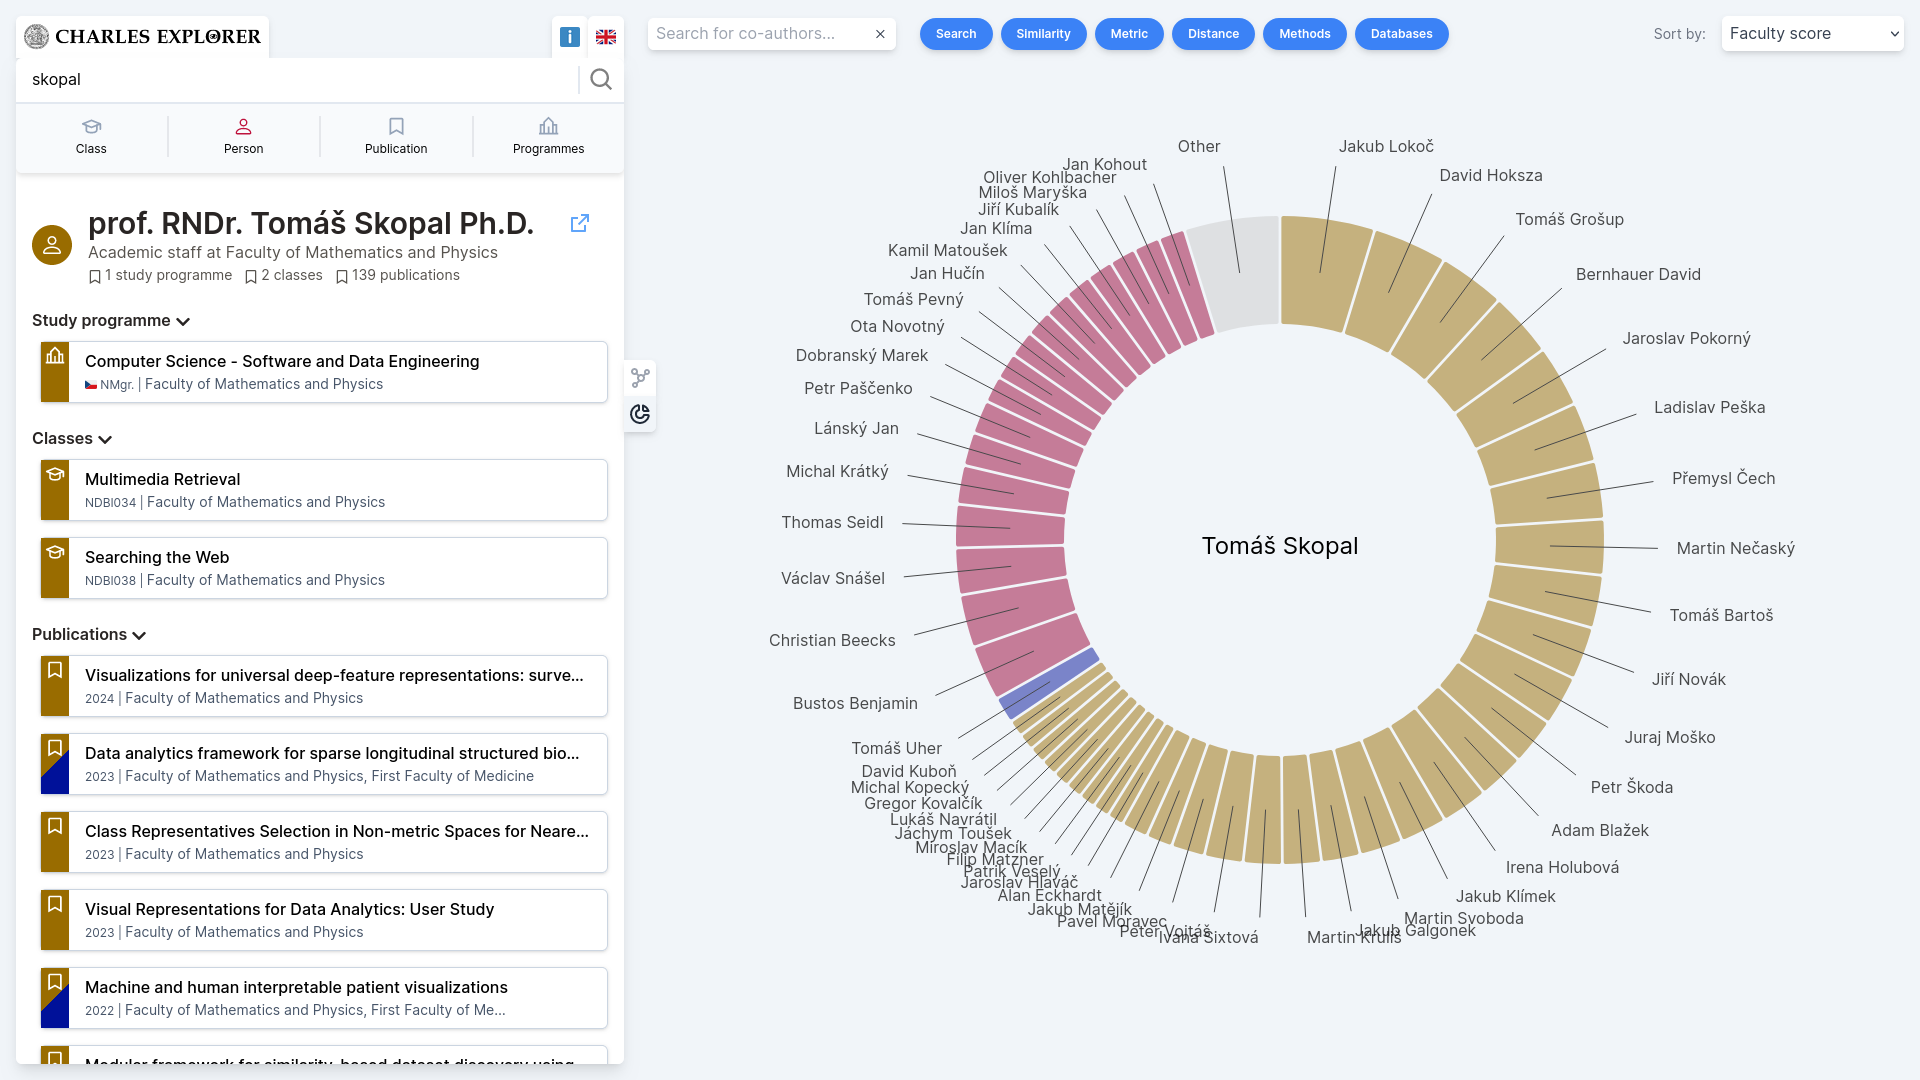
\includegraphics[width=0.8\textwidth]{../img/pie-chart.png}
    \centering
    \caption{The \textit{pie chart} view shows the distribution of faculty affiliations in the ego network, as well as the most frequent collaborators of the ego.}
\end{figure}

This visualization is still suffering from some of the problems of the original one. 

A publication with $n$ authors still contributes to $(n-1)$ pie chart arcs. 
This causes the solo publications to not be represented in the pie chart at all, and the publications with more than two authors to be overrepresented.

The color coding of the pie chart arcs (denoting the faculty affiliation) is also not ideal, since it still poses a problem for color vision deficient users.

For addressing these issues, we add few more features to the pie chart view.

Firstly, we reuse the tooltip user interface element from the graph view. 
When the user hovers over the pie chart arc, they can see the faculty affiliation name and the number of co-authored publications.

This helps both the color vision deficient users with identifying the faculty affiliation, and the general users with understanding the scale of the collaboration.

Secondly, we add an on-click boolean \texttt{AND} filter. 
When the user clicks on the pie chart arc, the view filters the underlying data to only represent co-authors of both the ego and the clicked-on co-author.

\begin{figure}[ht!]
    \captionsetup{width=.9\linewidth}
    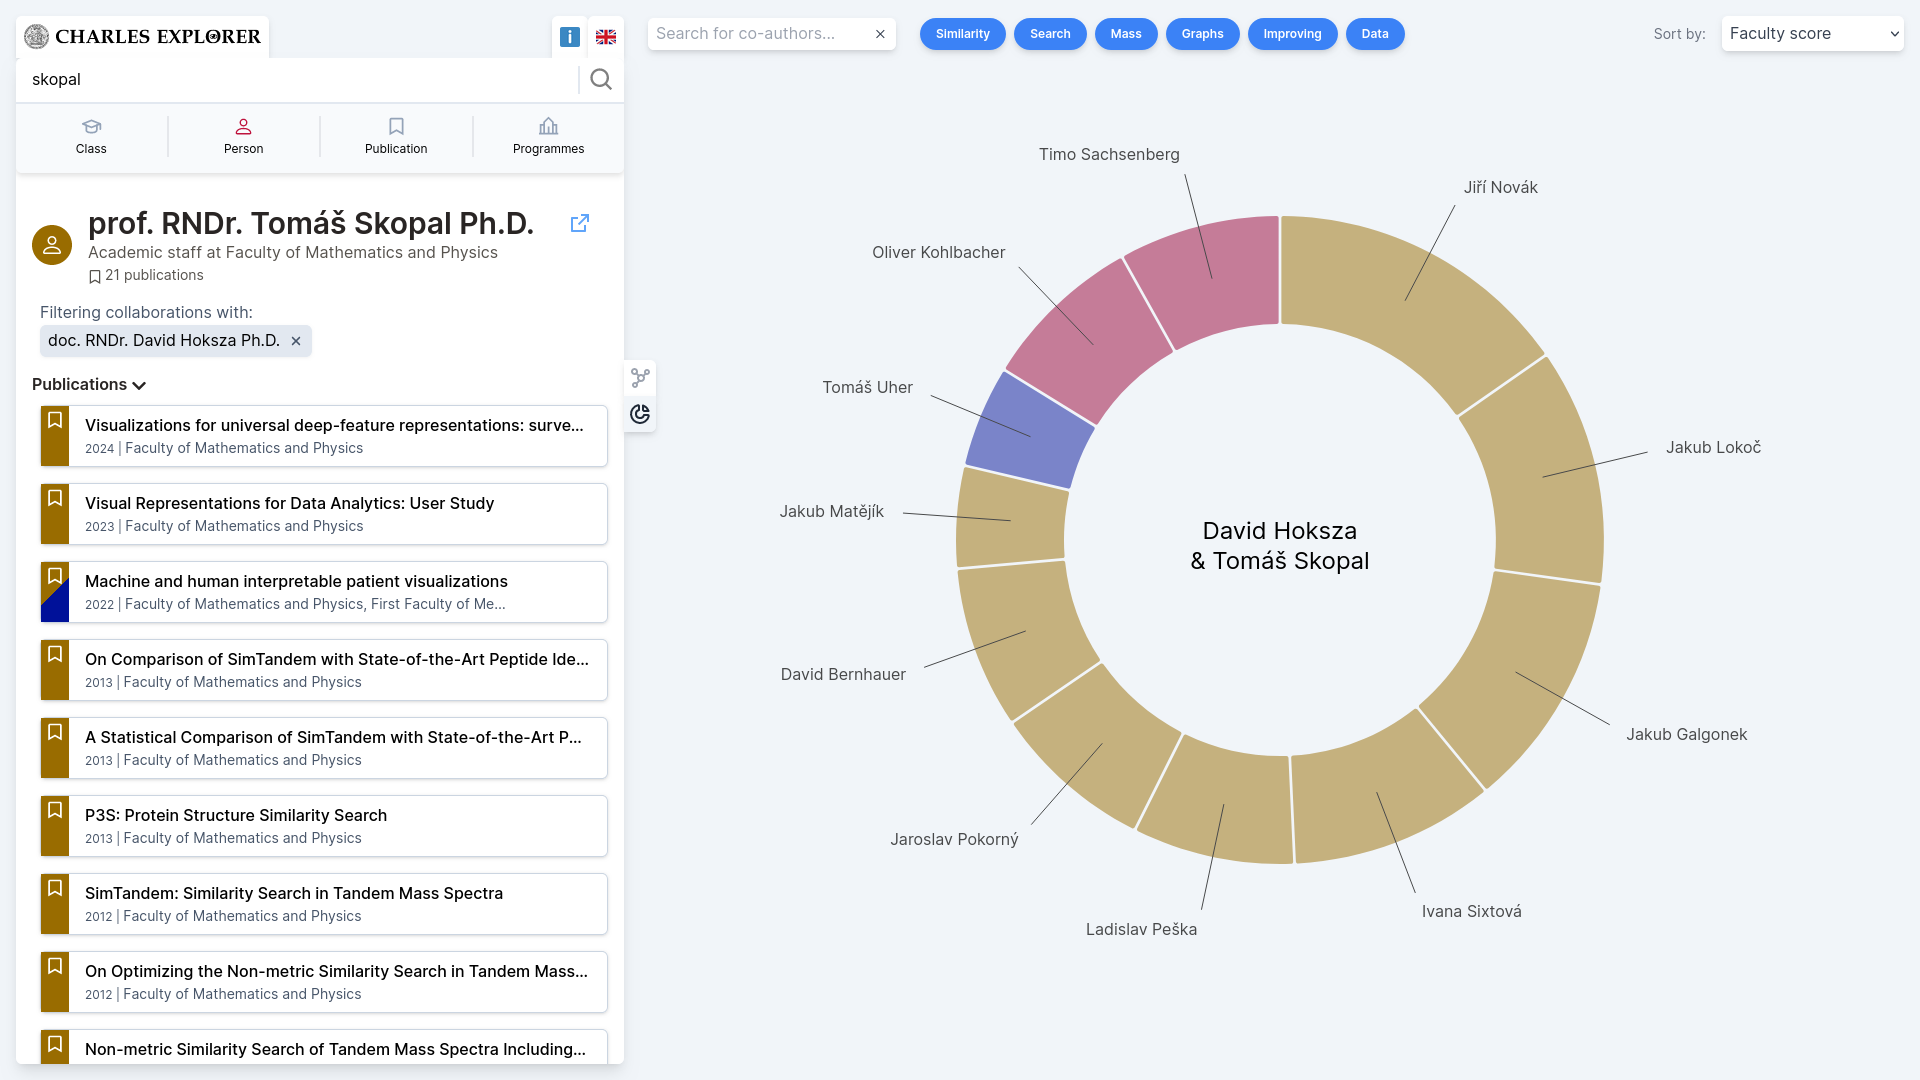
\includegraphics[width=0.8\textwidth]{../img/pie-chart-filter.png}
    \centering
    \caption{Right-clicking on the pie chart arc shows intersection of the ego's and the clicked-on person's collaborators.}
\end{figure}

The \texttt{AND} filter can be used repeatedly, adding new ``pinned'' collaborators one at a time.
Focusing on a smaller subset of the ego network can help to mitigate the problems with the overrepresentation of the publications with more than two authors
help the user to understand the smaller-scale collaboration patterns better.

The filter also applies to the left side of the view, where the user can see the actual publications of the selected co-authors.
This further clears up the multiple co-authorship problem.

% \section{Graph layouting algorithms}

% Before we start, let us introduce some basic terminology that will be used throughout this chapter.

% A \emph{graph layout} is a way to position the nodes of a graph in a two-dimensional space, such as on a screen or in print. 
% This is a necessary step of any graph data visualisation task - without computing the layout, the graph nodes nor edges do not have any intrinsic location assigned to them.

% There are several various ways of computing the graph layout, which we'll describe now in no particular order:

% \begin{itemize}
%     \item \textbf{Hierarchical layout} - for certain types of graphs, it's beneficial to display them in a hierarchical manner. 
%     This is usually the case for trees, i.e. connected acyclic graphs - such as family trees or organisation structures.

%     Such layout is typically laid out on either horizontal or vertical axis, with the root node at the top or leftmost position, and the children nodes below or to the right of their parent nodes.
%     The other direction (i.e. vertical for horizontal-major graphs and vice versa) is used for layouting the incomparable sibling groups.
    
%     While this layout might be used on cyclic graphs as well, it's not as common, as it's not as easy to interpret for laymen as the other layouts.
%     It might be useful for graphs with some kind of hierarchy or other clear ``score'' quality, such as social networks with a clear leader, or a company structure.

%     \item \textbf{Circular layout} - this layout places the nodes on a circle, with the edges connecting them. 
%     This layout is useful for visualizing relations between members of a group or community, as it's easy to see which nodes are connected to which other nodes.
%     Some work can be done for calculating the optimal placement of nodes - be it minimizing the edge length, or minimizing the number of edge crossings.

%     While minimizing the number of edge crossings might help with the graph readability, it might result in a less visually appealing graph, as the nodes might be placed further apart than necessary.
%     % TODO: add a reference to the paper about this.

%     Trying to minimize the edge length by ordering the nodes on the circle also results in a more readable graph, as this layout promotes grouping closely connected subcommunities together.

%     In some cases, the global position of nodes in the layout can depict some qualitative variable - e.g. in a social network of people from different social groups, 
%     the node position on the y-axis might represent the person's annual income. With the edges between the nodes representing the social connections,
%     such layout can help us understand the relation between the social status and the connections between the people.

%     \item \textbf{Grid layout} - this layout places the nodes on a grid, with the edges connecting them.
%     While some optimizations, such as minimizing the edge length can be done in this case as well, 
%     this type of layout usually results in a less readable graph.

%     An equally-spaced grid layout only communicates the relations between nodes by drawing the edges between them, not utilising the position of the nodes.
%     It is often the spatial proximity of the nodes that helps viewers understand the relations between the nodes subconciously - and while we still can 
%     supply this information by using different visual cues (e.g. coloring of the nodes), it's often not as intuitive as the spatial proximity.

%     Unlike the hierarchical and circular layouts, there does not seem to be a clear use for the global node position for depicting some qualitative variable.

%     In some applications, the grid layout is sometimes used as the initial graph layout for the force-directed layout, as it's easier to calculate the initial positions of the nodes on a grid.

%     \item \textbf{Force-directed layout} - this layout is based on the physical simulation of the forces between the nodes and edges of the graph.
%     The nodes are treated as charged particles, and the edges as springs - the nodes repel each other, while the edges try to keep the nodes connected.
    
%     This results in a layout where the nodes are placed in such a way that the edges are as short as possible, while the nodes are as far apart as possible.
%     This is useful for visualizing the overall structure of the graph, as it's easy to see which nodes are connected to which other nodes, and how the graph is connected.

%     Using the edges to guide the layouting process results in a more ``intuitively'' readable graph, as the edges representing some sort of relation between two nodes 
%     cause the nodes to be drawn to each other. This means that related nodes are layouted closer to each other - therefore supporting the spatial proximity Gestalt principle.

%     The force-directed layout is especially useful for visualizing large social networks, as it's easy to see which nodes are connected to which other nodes, and how the graph is connected.
%     Such graph is also easy to navigate, and the viewer can easily find bridges, hubs, or other important features of the graph.

%     Similar to the grid layout, the global node position cannot be used to depict qualitative variables. While it might be technically possible 
%     to add auxiliary forces to the simulation to achieve this - e.g. pull nodes to the left or right of the screen based on some variable - 
%     it's not as common as in the hierarchical or circular layouts. This approach might also interfere with the edge-based layouting process,
%     causing the graph to be less readable.

%     Because of this reason and the very essence of the force-directed layouts, the location of the nodes in such layout is quite arbitrary 
%     - in case of large graphs, the viewer might not be able to find the node they are looking for. This is why it's often useful to add 
%     some sort of search functionality or other navigation aids to the visualization.
% \end{itemize}
